% User manual of yaehmop-bandfit
% Build (inside manual/):  latexmk -pdf manual.tex   (or: pdflatex manual.tex twice)
% Source of the content: the Markdown files in ../docs, the code in ../parameter_fitter and ../USER_WORKFLOW.
\documentclass[11pt,a4paper]{article}

\usepackage[T1]{fontenc}
\usepackage[utf8]{inputenc}
\usepackage[english]{babel}
\usepackage{lmodern}
\usepackage{microtype}
\DisableLigatures[-]{encoding=T1,family=tt*}  % keep "--flag" as two hyphens
\usepackage[a4paper,margin=2.3cm,headheight=14pt]{geometry}
\usepackage{graphicx}
\usepackage[table]{xcolor}
\usepackage{booktabs}
\usepackage{tabularx}
\usepackage{array}
\usepackage{amsmath}
\usepackage{enumitem}
\usepackage{titlesec}
\usepackage{fancyhdr}
\usepackage{listings}
\usepackage[most]{tcolorbox}
\usepackage{tikz}
\usetikzlibrary{positioning,arrows.meta,shapes.geometric}
\usepackage[hidelinks]{hyperref}

\graphicspath{{../assets/}}

\definecolor{azul}{HTML}{1F4E79}
\definecolor{verm}{HTML}{D9534F}
\definecolor{cinza}{HTML}{F4F6F8}
\definecolor{borda}{HTML}{C9D3DD}

\titleformat{\section}{\Large\bfseries\color{azul}}{\thesection}{0.6em}{}
\titleformat{\subsection}{\large\bfseries\color{azul}}{\thesubsection}{0.6em}{}
\pagestyle{fancy}\fancyhf{}
\fancyhead[L]{\raisebox{-0.25\height}{
\includegraphics[height=12pt]{logo/bandfit_icon.pdf}}\hspace{4pt}\small\color{gray}YAeHMOP BandFit --- user manual}
\fancyhead[R]{\small\color{gray}\thepage}
\renewcommand{\headrulewidth}{0.3pt}

\lstset{basicstyle=\ttfamily\small,backgroundcolor=\color{cinza},frame=single,rulecolor=\color{borda},
  breaklines=true,columns=fullflexible,keepspaces=true,showstringspaces=false,
  literate={Γ}{{$\Gamma$}}1 {×}{{$\times$}}1 {→}{{$\rightarrow$}}1 {≥}{{$\geq$}}1 {│}{{|}}1 {▼}{{v}}1}
\lstdefinestyle{sh}{language=bash,keywordstyle=\color{azul}\bfseries,commentstyle=\color{gray}\itshape}
\lstdefinestyle{ini}{commentstyle=\color{gray}\itshape,morecomment=[l]{\#}}

\newtcolorbox{nota}[1][Note]{colback=azul!5,colframe=azul!60,title=#1,fonttitle=\bfseries,boxrule=0.6pt,arc=2pt}
\newtcolorbox{aviso}[1][Warning]{colback=verm!5,colframe=verm!70,title=#1,fonttitle=\bfseries,boxrule=0.6pt,arc=2pt}
\newcommand{\cmd}[1]{\texttt{#1}}
\setlength{\emergencystretch}{3em}
\tolerance=1500
\let\origunderscore\_
\renewcommand{\_}{\origunderscore\allowbreak}
\newcolumntype{L}{>{\raggedright\arraybackslash}X}

\begin{document}

% ---------------------------------------------------------------- title page
\begin{titlepage}
\centering
\vspace*{1.6cm}

\includegraphics[width=0.82\textwidth]{logo/bandfit_logo_dark.pdf}\par
\vspace{1.0cm}
{\Large Fitting physical extended H\"uckel parameters to reference band structures\par}
\vspace{0.4cm}
{\large 2, 4, 6 or 8 bands \,$\cdot$\, direct fit \,$\cdot$\, frozen transfer \,$\cdot$\, family fit\par}
\vspace{1.5cm}
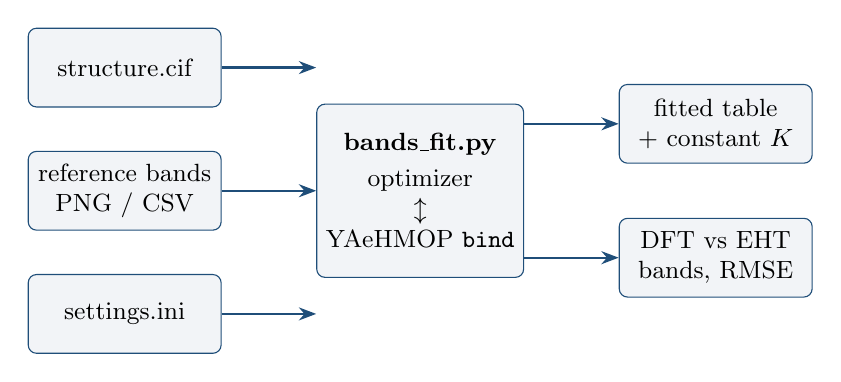
\begin{tikzpicture}[node distance=0.55cm and 0.55cm,
  box/.style={draw=azul,fill=azul!6,rounded corners=3pt,minimum width=2.45cm,minimum height=1.0cm,
              align=center,font=\small},
  arr/.style={-{Stealth[length=2.2mm]},thick,azul}]
\node[box] (cif) {structure.cif};
\node[box,below=of cif] (ref) {reference bands\\PNG / CSV};
\node[box,below=of ref] (ini) {settings.ini};
\node[box,right=1.2cm of ref,minimum height=2.2cm] (fit) {\textbf{bands\_fit.py}\\[2pt]optimizer\\$\updownarrow$\\YAeHMOP \cmd{bind}};
\node[box,right=1.2cm of fit,yshift=0.85cm] (par) {fitted table\\+ constant $K$};
\node[box,right=1.2cm of fit,yshift=-0.85cm] (bands) {DFT vs EHT\\bands, RMSE};
\draw[arr] (cif.east) -- (fit.west|-cif.east);
\draw[arr] (ref) -- (fit);
\draw[arr] (ini.east) -- (fit.west|-ini.east);
\draw[arr] (fit.east|-par.west) -- (par.west);
\draw[arr] (fit.east|-bands.west) -- (bands.west);
\end{tikzpicture}
\vfill
{\large User manual\par}
\vspace{0.2cm}
{\small Built from the repository documentation (\cmd{docs/}) and source code, branch \cmd{adias-dev}.\par}
{\small \today\par}
\end{titlepage}

\tableofcontents
\newpage

% ================================================================ 1
\section{What the program does}

YAeHMOP BandFit adjusts the atomic parameters of the \textbf{extended H\"uckel theory} (EHT) so that the
band structure computed by the original YAeHMOP solver reproduces a reference band structure, usually from
DFT. You give a crystal structure (CIF, or a VASP, Quantum ESPRESSO, SIESTA or FHI-aims file), the reference bands (an image or a numerical CSV) and a small INI
settings file. The program returns:

\begin{itemize}[nosep]
  \item a parameter table in the native YAeHMOP format (\cmd{param\_best\_native.dat}) and the
        Wolfsberg--Helmholtz constant $K$, which run directly in the original \cmd{bind};
  \item the RMSE between reference and EHT bands and a comparison plot (PNG, PDF, CSV);
  \item on request, \textbf{all} EHT bands recomputed with the fitted parameters.
\end{itemize}

There is no surrogate or machine-learned Hamiltonian: \textbf{every evaluation of the objective is one real
YAeHMOP calculation}, with the full nonorthogonal orbital Hamiltonian. The image reader is only a bridge
that turns a plot into numbers.

\subsection{The three workflows}

\begin{center}
\begin{tabularx}{\textwidth}{>{\bfseries}l L L}
\toprule
Workflow & Question it answers & Command \\
\midrule
Direct fit & How well can EHT reproduce \emph{this} material? (calibration, in-sample) & \cmd{USER\_WORKFLOW/bands\_fit.py} \\
Frozen transfer & Do parameters fitted elsewhere predict \emph{another} material, with zero refitting? & \cmd{USER\_WORKFLOW/frozen\_transfer.py} \\
Family fit & Can \emph{one} parameter vector describe several training materials and a held-out one? & \cmd{USER\_WORKFLOW/family\_fit.py} \\
\bottomrule
\end{tabularx}
\end{center}

\begin{aviso}[Direct fit is not transfer]
A direct fit sees the target while optimizing, so its error measures representability, not prediction.
Never pool direct-fit errors with held-out (transfer) errors.
\end{aviso}

\subsection{Selected bands: 1V+1C to 4V+4C}

The fit always compares \textbf{N selected reference bands with N EHT eigenvalues}: the $N/2$ highest
valence and the $N/2$ lowest conduction bands around the gap. \cmd{--pairs 1} means 1V+1C (2 bands),
\cmd{--pairs 2} means 2V+2C (4 bands), and so on up to \cmd{--pairs 4} (8 bands). YAeHMOP still
diagonalizes the whole orbital basis; the other bands are simply not part of the objective. Use more
pairs only when the reference really contains that many identifiable bands.

% ================================================================ 2
\section{Installation}

\subsection{Automatic installation: \cmd{install.sh}}

The script creates (or updates) the conda environment from \cmd{environment.yml}, checks the Python
packages, configures YAeHMOP and runs one real test calculation:

\begin{lstlisting}[style=sh]
git clone https://github.com/tromer-unb/yaehmop-bandfit.git
cd yaehmop-bandfit
./install.sh --build-yaehmop --tests     # also downloads and compiles YAeHMOP into the environment
conda activate yaehmop-bandfit
\end{lstlisting}

\begin{center}
\begin{tabularx}{\textwidth}{>{\ttfamily}l L}
\toprule
\normalfont Option & Effect \\
\midrule
--env NAME & environment name (default \cmd{yaehmop-bandfit}) \\
--build-yaehmop & clone upstream YAeHMOP (commit \cmd{4ded45b} by default, change with \cmd{--yaehmop-ref}), compile it with the conda compiler and OpenBLAS, install \cmd{bind} and \cmd{eht\_parms.dat} inside the environment \\
--yaehmop-bind, --yaehmop-params & use a YAeHMOP that is already installed \\
--tests & run the test suite at the end \\
\bottomrule
\end{tabularx}
\end{center}

In both cases \cmd{YAEHMOP\_BIND} and \cmd{YAEHMOP\_PARAM\_FILE} are stored in the environment and set
on \cmd{conda activate}. Without these options the values already exported in the shell are kept. The
script uses the fast \cmd{libmamba} solver when available.

\subsection{Python environment by hand}

Two options. With conda, using the \cmd{environment.yml} at the repository root (it also installs the
optional packages of the Bayesian and CMA-ES optimizers):

\begin{lstlisting}[style=sh]
git clone https://github.com/tromer-unb/yaehmop-bandfit.git
cd yaehmop-bandfit
conda env create -f environment.yml
conda activate yaehmop-bandfit
\end{lstlisting}

Or with a plain virtual environment:

\begin{lstlisting}[style=sh]
python3 -m venv .venv
source .venv/bin/activate
python -m pip install -r requirements.txt
python quick.py          # saved paper figures, no physics calculation
\end{lstlisting}

Python 3.10 or newer is recommended (Linux or macOS). Dependencies: \cmd{numpy}, \cmd{scipy}, \cmd{ase},
\cmd{Pillow}, \cmd{matplotlib}, \cmd{PyYAML}; optionally \cmd{scikit-learn} (optimizer \cmd{bayesian})
and \cmd{cma} (optimizer \cmd{cmaes}).

\subsection{YAeHMOP}

The solver and its atomic parameter table are \textbf{not bundled}. Build YAeHMOP from its upstream
project (\url{https://github.com/greglandrum/yaehmop}, directory \cmd{tightbind}, CMake) or install it
from conda-forge, then point the program to it:

\begin{lstlisting}[style=sh]
export YAEHMOP_BIND=/absolute/path/to/bind
export YAEHMOP_PARAM_FILE=/absolute/path/to/eht_parms.dat
test -x "$YAEHMOP_BIND" && test -f "$YAEHMOP_PARAM_FILE"
\end{lstlisting}

With conda the variables can be stored in the environment once:
\cmd{conda env config vars set -n yaehmop-bandfit YAEHMOP\_BIND=... YAEHMOP\_PARAM\_FILE=...}.
The program calls \cmd{bind input\_file parameter\_file}; the upstream \cmd{bind} accepts the parameter
table as its second argument.

\begin{aviso}[\cmd{bind} is also a bash builtin]
Typing \cmd{bind file} in an interactive bash runs the shell builtin, not YAeHMOP. The program always
calls the executable by its full path, so this only matters when you run YAeHMOP by hand: use the full
path or a link with another name.
\end{aviso}

\subsection{What needs the solver}

Inspecting images, preparing references, plotting saved results, \cmd{quick.py} and the test suite
(\cmd{python -m unittest discover -s tests}) do \textbf{not} need YAeHMOP. Only fitting, frozen
evaluation and recomputation of bands run it. GitHub Actions run only the light tests.

% ================================================================ 3
\section{Inputs}

\subsection{Crystal structure}\label{sec:structure}

The structure can be a CIF or the structure file of one of four DFT packages. The format is detected from
the file name and, when that is not conclusive, from the content; \cmd{--structure-format} forces it
(\cmd{structure\_format:} in YAML manifests, per system or under \cmd{shared:}). The same crystal gives the
same YAeHMOP input in every format (tested to $10^{-6}$ against the CIF, including real YAeHMOP runs).

\begin{center}
\small
\begin{tabularx}{\textwidth}{l L >{\ttfamily}l}
\toprule
Package & Files & \normalfont\cmd{--structure-format} \\
\midrule
--- & \cmd{*.cif} & cif \\
VASP & \cmd{POSCAR}, \cmd{CONTCAR}, \cmd{*.vasp}; \cmd{OUTCAR}; \cmd{vasprun.xml} & vasp, vasp-out, vasp-xml \\
Quantum ESPRESSO & pw.x input (\cmd{*.pwi}, \cmd{*.in}, any \cmd{ibrav}); output (\cmd{*.pwo}) & qe, qe-out \\
SIESTA & \cmd{*.fdf}; \cmd{*.XV}; \cmd{*.STRUCT\_OUT} & siesta, siesta-xv, siesta-struct-out \\
FHI-aims & \cmd{geometry.in}; output & aims, aims-out \\
\bottomrule
\end{tabularx}
\end{center}

ASE does the parsing, except where it cannot: the SIESTA \cmd{.fdf} (\cmd{LatticeConstant},
\cmd{LatticeVectors} or \cmd{LatticeParameters}, \cmd{ChemicalSpeciesLabel}, all
\cmd{AtomicCoordinatesFormat} values, \cmd{AtomicCoordinatesAndAtomicSpecies}, \cmd{\%include}) and the
pw.x lattice for $\text{ibrav}\neq 0$ (vectors as in QE \cmd{latgen}, from \cmd{celldm} or
\cmd{A}, \cmd{B}, \cmd{C}, \cmd{cosAB}\ldots) are read by \cmd{parameter\_fitter/structure\_io.py}. Output
files give the last (relaxed) geometry. The file must contain a full $3\times3$ cell (vacuum vector included
for 2D/1D materials), and the \cmd{[band\_path]} points refer to \emph{its} reciprocal vectors.
Z-matrix and ghost atoms in SIESTA and \cmd{crystal\_sg} in QE are not supported. Details in
\cmd{docs/STRUCTURE\_FORMATS.md}.

\subsection{The settings file (INI)}

\begin{lstlisting}[style=ini]
[reference]
image = bands.png          # or bands.csv; path relative to this INI file
mode = auto                # auto | colors | mono | layered | csv
emin = -6                  # energy at the BOTTOM of the plot frame (eV)
emax = 6                   # energy at the TOP of the plot frame (eV)
trace_nx = 301
min_coverage = 0.80

[band_path]
dimension = 2              # 2 for layers, 3 for bulk crystals (also the lattice periodicity)
points = 0,0; 0.5,0; 0.3333333333,0.3333333333; 0,0
labels = G,M,K,G
points_per_segment = 20

[fit]
n_pairs = 1                # 1V+1C; 2, 3, 4 only with a real multi-band reference
budget = 400               # number of YAeHMOP calls
optimizer = nelder-mead
gap_weight = 0.35
reg_weight = 0.04
# overlap_radius = 5       # periodic images per active direction (default 5)
# polish = nelder-mead     # only after a global optimizer
\end{lstlisting}

\begin{itemize}[nosep]
  \item \textbf{emin/emax} are the energies of the plot frame, not the band extrema.
  \item \textbf{points/labels} are fractional reciprocal coordinates of \emph{that} CIF along \emph{that}
        DFT path. With \cmd{dimension = 3} each node has three coordinates.
  \item \textbf{dimension} also sets the periodicity written for YAeHMOP (\cmd{Lattice 2} or
        \cmd{Lattice 3}); see section~\ref{sec:lattice}.
\end{itemize}

\subsection{Raw DFT band data (VASP, QE, SIESTA, FHI-aims)}\label{sec:dft}

The reference can be the folder of a DFT band-structure calculation. The eigenvalues, the k points, the
structure and the number of occupied bands are read from the files; no image is involved:
\begin{lstlisting}[style=sh]
python USER_WORKFLOW/bands_fit.py settings.ini --dft-dir path/to/bands --dft-code vasp \
  --outdir outputs/material
\end{lstlisting}
The INI file needs only \cmd{[fit]} (template \cmd{examples/configs/dft\_template.ini}); the structure argument is
optional (the DFT structure is used).

\begin{center}
\small
\begin{tabularx}{\textwidth}{l L L}
\toprule
Code & Eigenvalues and k points & Occupied bands / labels \\
\midrule
VASP & \cmd{vasprun.xml} or \cmd{EIGENVAL} (+ \cmd{POSCAR}) & \cmd{NELECT}; line-mode \cmd{KPOINTS} \\
QE & XML of the \cmd{bands} run, pw.x output, or \cmd{bands.x} file & \cmd{nelec}; \cmd{crystal\_b} with \cmd{! label} \\
SIESTA & \cmd{.bands} + \cmd{.fdf} with \cmd{BandLines} & Fermi level; \cmd{BandLines} \\
FHI-aims & \cmd{band1001.out}\ldots{} + \cmd{control.in} & occupations; \cmd{output band} \\
\bottomrule
\end{tabularx}
\end{center}

Each straight DFT segment becomes a YAeHMOP band line (\cmd{points\_per\_segment} points) and the DFT
eigenvalues are interpolated at exactly those k points; discontinuities (\cmd{X|U}) are computed but excluded
from the error. The periodic dimension is detected from the vacuum unless given. Spin--orbit and
spin-polarized (different channels) references and metals are refused; FHI-aims \cmd{*.no\_soc} files are used
when present. \cmd{--from-fit} or \cmd{--from-parameters} with \cmd{--dft-dir} evaluate existing parameters.
Details in \cmd{docs/DFT\_REFERENCE.md}; real examples in \cmd{validation/}.

Every fit, with any reference, writes the standard output folder described in
section~\ref{sec:outputs}.

\subsection{Numerical CSV (preferred reference)}

A CSV avoids every ambiguity of a raster image. The header must be exactly
\cmd{x,band\_1,...,band\_N} with $N = 2, 4, 6$ or $8$:

\begin{lstlisting}
x,band_1,band_2
0.0,-1.15,1.22
0.1,-1.18,1.30
...
\end{lstlisting}

\begin{itemize}[nosep]
  \item \cmd{x}: normalized path coordinate, strictly increasing from 0 to 1 (not \AA$^{-1}$);
  \item energies in eV, ascending in every row, all finite, inside \cmd{emin}/\cmd{emax};
  \item at least 15 rows; the frontier gap must be positive (above about 0.02~eV).
\end{itemize}

Do not confuse it with the saved full-orbital EHT files in \cmd{examples/precomputed/} (columns
\cmd{x,kx,ky,kz,orbital\_1,...}): those are model outputs for plotting, not references.

\subsection{Images}

Any still raster that Pillow decodes (PNG, JPEG, TIFF, BMP, WebP, single-frame GIF, PPM) is accepted;
the format is detected from the content, not the extension. The reading pipeline is:

\begin{enumerate}[nosep]
  \item decode and validate (one frame, size limits, EXIF orientation, color profile, SHA-256);
  \item write \cmd{normalized\_source.png} and \cmd{raster\_ingest\_qa.json};
  \item find the curves: \cmd{colors} (one hex color per band, in energy order), \cmd{auto}
        (conservative detection), \cmd{mono} (single-color heuristic) or \cmd{layered} (an already
        encoded bitplane image);
  \item check coverage, gap and interpolation, and write the internal \cmd{bands\_N\_layers.png},
        \cmd{extracted\_curves.csv}, \cmd{extraction\_qa.json} and \cmd{extraction\_preview.png}.
\end{enumerate}

\begin{lstlisting}[style=sh]
python USER_WORKFLOW/inspect_png.py bands.png --outdir outputs/inspect     # suggests bbox and colors
python USER_WORKFLOW/prepare_band_png.py bands.png --mode colors --n-pairs 1 \
  --emin -6 --emax 6 --bbox 110,80,920,650 --colors '#c82d37,#1c7ad5' --outdir outputs/prepared
\end{lstlisting}

\begin{aviso}[Always look at the preview]
Open \cmd{extraction\_preview.png} before fitting. A screenshot cannot reveal hidden or overlapping
bands; the program never invents missing curves. When tracing is doubtful, use a CSV or the manual
digitizer (\cmd{USER\_WORKFLOW/digitize\_bands.py}).
\end{aviso}

\subsection{The internal bitplane PNG}

All references are converted to one format: an 8-bit grayscale PNG (canvas $3200\times3400$, plot box
\cmd{(160,100,3000,3260)}) where each band occupies one bit. Two bands at the same pixel add their bits,
so recorded crossings are preserved.

\begin{center}
\begin{tabular}{rl}
\toprule
Pixel value & Meaning (N = 4) \\
\midrule
0 & no band \\
1, 2, 4, 8 & band 1, 2, 3, 4 alone (band 1 lowest) \\
5 = 1 + 4 & bands 1 and 3 at the same pixel \\
\bottomrule
\end{tabular}
\end{center}

The round-trip error reported in the QA measures only this encoding, not the accuracy of the original
digitization or of the DFT.

% ================================================================ 4
\section{Direct fit, step by step}

\subsection{1. Prepare and check the reference (no solver)}

\begin{lstlisting}[style=sh]
mkdir -p inputs/my_material
cp /path/structure.cif inputs/my_material/structure.cif
cp /path/bands.png     inputs/my_material/bands.png
cp examples/configs/material_2bands_template.ini inputs/my_material/file.ini
# edit file.ini: real emin/emax, k path, labels, band count

python USER_WORKFLOW/bands_fit.py inputs/my_material/structure.cif \
  inputs/my_material/file.ini --prepare-only --outdir outputs/my_material
\end{lstlisting}

\subsection{2. Fit}

\begin{lstlisting}[style=sh]
python USER_WORKFLOW/bands_fit.py inputs/my_material/structure.cif \
  inputs/my_material/file.ini --pairs 1 --budget 400 --outdir outputs/my_material
\end{lstlisting}

\begin{center}
\begin{tabularx}{\textwidth}{>{\ttfamily}l L}
\toprule
\normalfont Output & Contents \\
\midrule
bands\_comparison.png/.pdf/.csv & reference versus the selected EHT bands \\
fit/param\_best\_native.dat & fitted table in native YAeHMOP format \\
fit/fit.json & parameters, $K$, metrics, optimizer state, lattice used \\
fit/history.csv & every objective evaluation \\
run\_summary.json & RMSE, gap error, $K$, hashes of the inputs, settings \\
\bottomrule
\end{tabularx}
\end{center}

\subsection{3. Recompute all bands}

\begin{lstlisting}[style=sh]
python USER_WORKFLOW/bands_fit.py inputs/my_material/structure.cif \
  inputs/my_material/file.ini --from-fit outputs/my_material/fit/fit.json \
  --outdir outputs/my_material_full
\end{lstlisting}

This writes \cmd{bands\_full.png/.pdf/.csv/.npz} with \textbf{every} orbital eigenvalue (the plot
shows only the chosen energy window). The CIF is checked by SHA-256 against the fit. With a table of
your own use \cmd{--from-parameters table.dat --k VALUE} instead.

\subsection{Output files}\label{sec:outputs}

Every fit of \cmd{bands\_fit.py} (DFT, image or CSV reference, and also \cmd{--from-fit} /
\cmd{--from-parameters} with \cmd{--dft-dir}) writes \cmd{OUTDIR/fitting/} (or the folder given with
\cmd{--fitting-dir}). Everything is plain text except the figures.

\begin{center}
\small
\begin{tabularx}{\textwidth}{>{\ttfamily}l L}
\toprule
\normalfont File & Content \\
\midrule
parameters\_huckel.dat & fitted parameters in the native YAeHMOP table format; usable directly as
  \cmd{bind input.bind parameters\_huckel.dat} \\
parameters\_huckel.txt & $K_{\rm EHT}$ and every fitted variable (\cmd{name value}) \\
fit\_summary.json & errors (RMSE, gap error, \ldots), optimizer and budget, reference and structure used,
  periodic dimension, EHT midgap $E_{\rm mid}$, checks of the exported matrices \\
bands\_comparison.png/pdf & fitted bands: reference in blue (solid), EHT in red (dashed), both relative to
  their midgap; RMSE, MAE, max $|\Delta E|$ and gaps (reference, EHT, error) below the plot \\
bands\_comparison.csv & the curves of that figure: \cmd{k, REF\_band\_1..N, EHT\_band\_1..N} \\
bands\_full\_comparison.* & (DFT references) all DFT and all EHT bands in the \cmd{[reference] emin/emax}
  window, with the same errors; \cmd{.csv} with every band \\
huckel-NP.dat & real-space Hamiltonian $H(\mathbf R)$ and overlap $S(\mathbf R)$ in the WanTiBEXOS
  non-orthogonal format (read with \cmd{DFT= S}) \\
basis\_set-NP & WanTiBEXOS basis file: \cmd{index species x y z l m spin} (positions in \AA) \\
orbitals.dat & orbital index, atom, orbital name, $l$, $m$, in YAeHMOP order \\
hamiltonian\_overlap\_k.dat & $H(\mathbf k)$ and $S(\mathbf k)$ at the high-symmetry points of the band
  figure (raw YAeHMOP values) \\
yaehmop\_matrices.bind & YAeHMOP input that produced the matrices (\cmd{K points}, \cmd{Dump Hamil/Overlap}) \\
POSCAR & the structure used (VASP format; exact cell and atomic order of the matrices) \\
README.txt & short description of these files \\
\bottomrule
\end{tabularx}
\end{center}

\paragraph{\cmd{huckel-NP.dat}.} Same layout as the files of \cmd{siesta2wtb.py}:
\begin{lstlisting}
NP                                  calculation type (spinless)
0.000000                            scissors (eV)
0.000000                            Fermi level (eV)
3.16288608  0.00000000  0.00000000  lattice vectors (A)
-1.58180956 2.73894467  0.00000000
0.00000000  0.00000000  16.00000000
17                                  number of basis orbitals (size of H and S)
101                                 number of hopping vectors R (cells)
#rcell x   rcell y   rcell z   i   j   ReH   ImH   S
-7.905  -13.695  0.000   1   1   -0.000187   0.000000   0.000012
...
\end{lstlisting}
For every vector $\mathbf R$ (Cartesian, \AA) and orbital pair $i,j$ (line order: $i$ outer, $j$ inner) it gives
$H_{ij}(\mathbf R)=\langle\phi_i(\mathbf 0)|H|\phi_j(\mathbf R)\rangle$ and $S_{ij}(\mathbf R)$, with
$H(\mathbf k)=\sum_{\mathbf R}e^{i\mathbf k\cdot\mathbf R}H(\mathbf R)$. YAeHMOP only writes $H(\mathbf k)$ and
$S(\mathbf k)$; since its lattice sums stop at the overlap radius $r$, $H(\mathbf R)$ and $S(\mathbf R)$ for all cells
$-r\ldots r$ are recovered exactly by a Fourier transform on the full $\Gamma$-centred mesh of $(2r+1)^{d}$ points
(cells whose elements are all below $10^{-7}$ are omitted). The column \cmd{ReH} holds
$H(\mathbf R)-E_{\rm mid}S(\mathbf R)$ and the Fermi level is 0: \cmd{wtb.x} diagonalizes $(H-E_F I, S)$, which is
not a rigid shift when $S\neq I$, so with this choice it reproduces the YAeHMOP bands relative to the EHT midgap
(checked for MoS$_2$: $10^{-4}$~eV near the gap). Add $E_{\rm mid}$ (\cmd{fit\_summary.json}) for absolute energies.
\cmd{ImH} is zero (real orbitals).

\paragraph{\cmd{basis\_set-NP} and \cmd{orbitals.dat}.} One line per orbital, in the order of the matrices:
s; $p_x,p_y,p_z$; $d_{x^2-y^2},d_{z^2},d_{xy},d_{xz},d_{yz}$; f. The $(l,m)$ follow sisl's real spherical
harmonics: $p_x$ $m{=}1$, $p_y$ $m{=}{-1}$, $p_z$ $m{=}0$; $d_{xy}$ $-2$, $d_{yz}$ $-1$, $d_{z^2}$ 0, $d_{xz}$ 1,
$d_{x^2-y^2}$ 2.

\paragraph{\cmd{hamiltonian\_overlap\_k.dat}.} The same header as \cmd{huckel-NP.dat}, but with the Fermi level
equal to the EHT midgap (absolute, since these $H(\mathbf k)$ are not shifted) and one more line with the number of
k points; then \cmd{k1 k2 k3 i j ReH ImH ReS ImS} with $\mathbf k$ in fractional reciprocal coordinates.

\paragraph{Other files in \cmd{OUTDIR}.} \cmd{fit/} (optimizer outputs: \cmd{fit.json}, \cmd{history.csv},
\cmd{param\_best\_native.dat}, band arrays), \cmd{fit\_input.yaml}, \cmd{run\_summary.json}; for DFT references
\cmd{dft\_reference/} (\cmd{POSCAR} of the DFT structure, \cmd{reference\_bands.npz}, \cmd{dft\_reference.json},
\cmd{dft\_bands\_preview.png}); for images \cmd{reference\_prepared/} (extraction QA).

% ================================================================ 5
\section{How the fit works}

\subsection{Parameters}

For each element and each orbital ($s$, $p$, $d$, $f$) present in the table:

\begin{center}
\begin{tabularx}{\textwidth}{l L L}
\toprule
Parameter & Meaning & Bounds in the main fitter \\
\midrule
$H_{ii}$ & on-site (Coulomb) energy & stock value $\pm 5$ eV \\
$\zeta_1$ & Slater exponent & $[\max(0.55,\,0.45\zeta),\ \min(9,\,2\zeta)]$ \\
$\zeta_2$ & second exponent (double-zeta orbitals only) & $[\max(0.45,\,0.45\zeta),\ \min(6,\,2\zeta)]$ \\
$c_2/c_1$ & ratio of the double-zeta coefficients & $[0.05,\ 2.5]$ \\
$K$ & global Wolfsberg--Helmholtz constant & $[1.0,\ 2.8]$ \\
\bottomrule
\end{tabularx}
\end{center}

Candidates with $\zeta_1 \le \zeta_2 + 0.12$ are rejected. The ratio is written as $c_1 = 1$,
$c_2 = \text{ratio}$: YAeHMOP normalizes the contracted orbital itself when it reads the table,
\begin{equation*}
  N = \bigl(c_1^2 + c_2^2 + 2c_1c_2S_{12}\bigr)^{-1/2},\qquad
  S_{12} = \left[\frac{4\zeta_1\zeta_2}{(\zeta_1+\zeta_2)^2}\right]^{n+1/2},
\end{equation*}
so only the ratio matters (checked numerically: scaling both coefficients leaves the eigenvalues
unchanged). In the stock solver only $d$ and $f$ orbitals are double-zeta; a carbon $2p$ double-zeta
needs the research patch in \cmd{experimental/}, applied to a separate copy of YAeHMOP.

\subsection{Objective}

The reference and the model are each aligned at their own mid-gap. Then
\begin{equation*}
  \text{loss} = \mathrm{RMSE}_{N\ \text{bands}} + w_\text{gap}\,|\Delta E_g| + w_\text{reg}\,R ,
\end{equation*}
with $w_\text{gap} = 0.35$, $w_\text{reg} = 0.04$ by default (\cmd{gap\_weight}, \cmd{reg\_weight}) and
$R$ the root-mean-square distance of the parameters from the stock table, each scaled by a typical
width. In a family fit the loss is the weighted mean over the training materials plus the same
regularization.

\subsection{Lattice and periodic images}\label{sec:lattice}

The input written for YAeHMOP uses \cmd{Lattice 2} or \cmd{Lattice 3} according to
\cmd{[band\_path] dimension}, with \cmd{overlap\_radius} periodic images (default 5) along each active
direction and zero along inactive ones. Fit and recomputation use the same values, which are stored in
\cmd{fit.json} and reused by \cmd{--from-fit} and \cmd{frozen\_transfer.py}. With 5 images the carbon
test bands are converged to about $10^{-5}$ eV (4 images leave errors near 1~meV).

\begin{aviso}[Fits made before the periodicity fix]
Older versions always wrote \cmd{Lattice 2} (images \cmd{5 5 0}) during the fit, even with
\cmd{dimension = 3}: a bulk crystal was fitted as a slab one cell thick, while the recomputation used
\cmd{Lattice 3}. \cmd{--from-fit} prints a warning for such \cmd{fit.json} files. Refit 3D materials.
\end{aviso}

\begin{figure}[h]
\centering
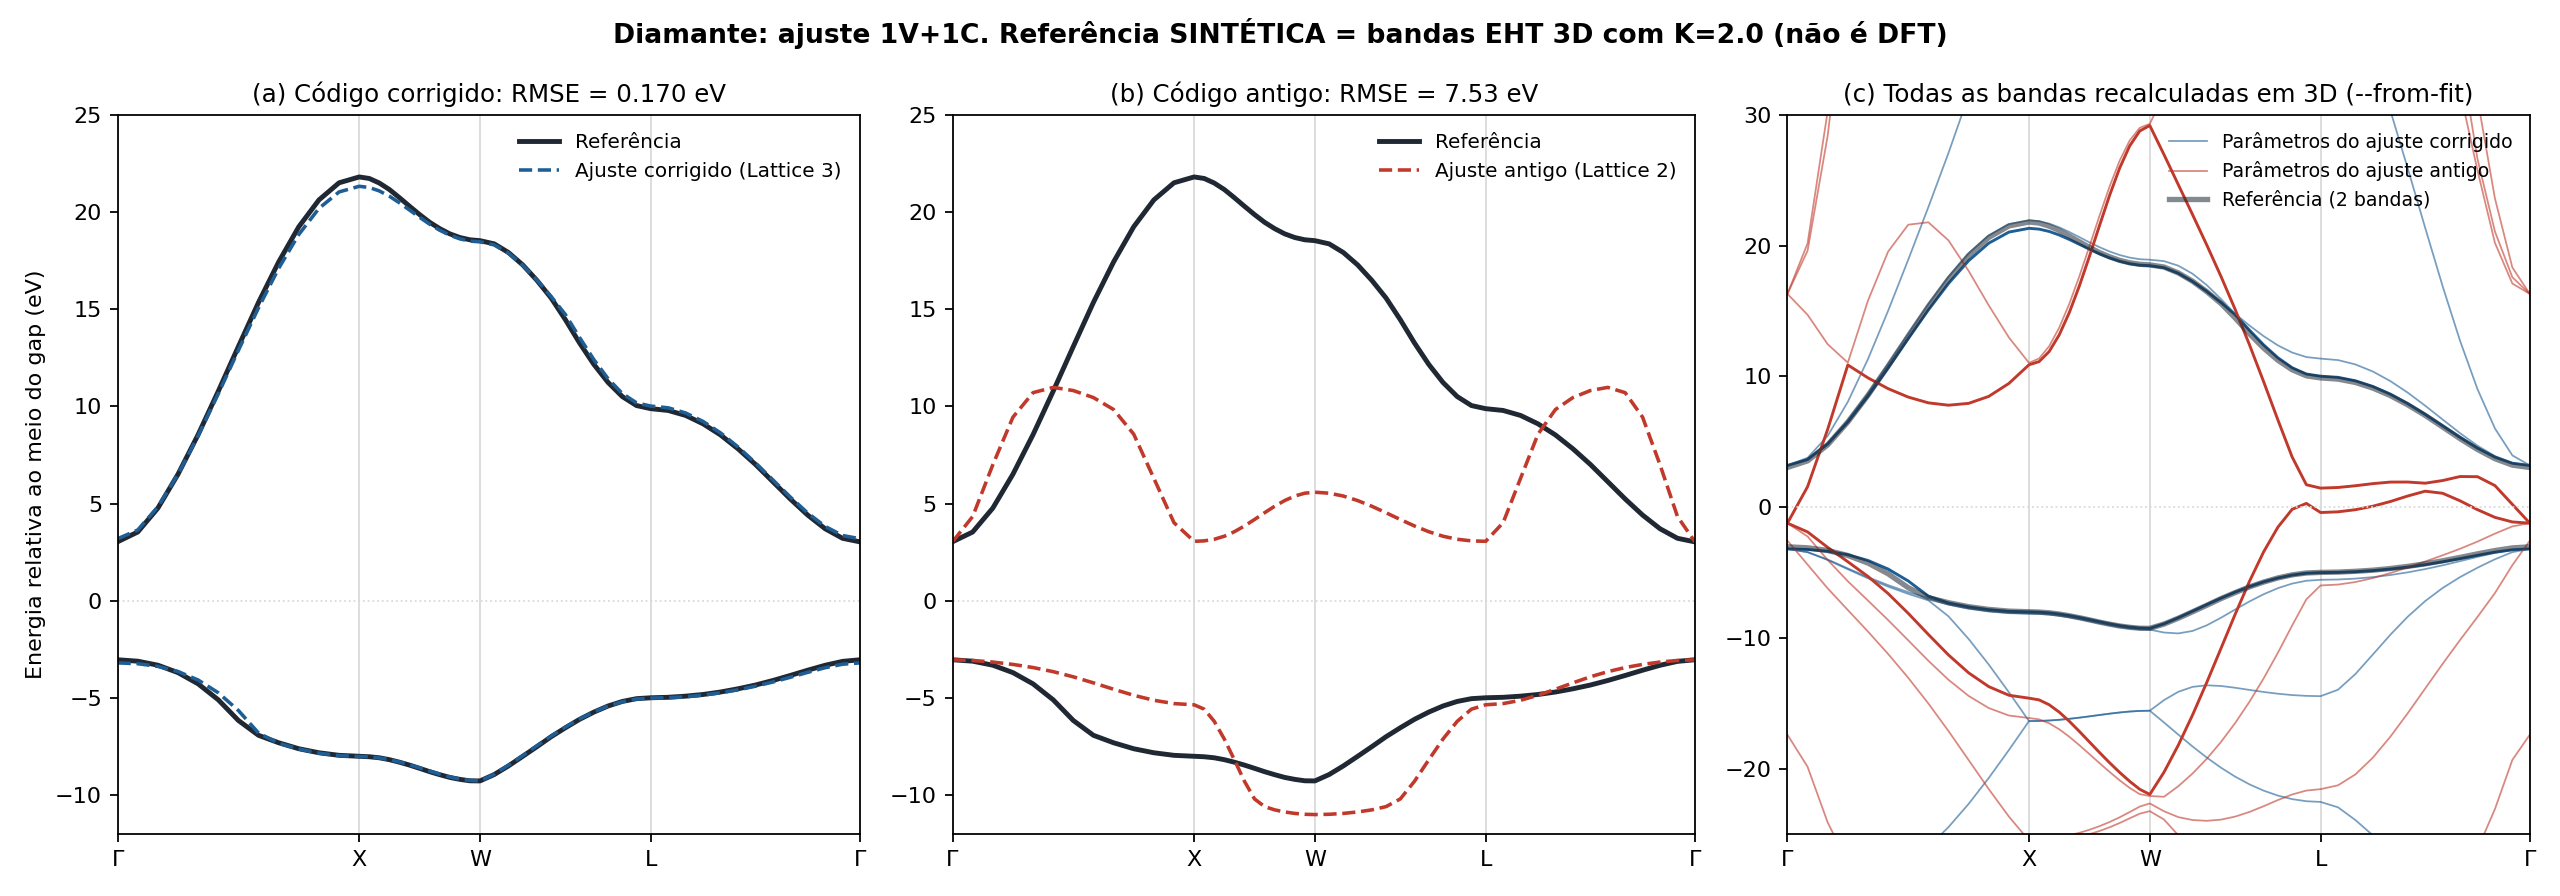
\includegraphics[width=\textwidth]{diamond_3d_periodicity_fix.png}
\caption{Diamond, 1V+1C, real YAeHMOP, 120 calls from the stock table, against a \emph{synthetic}
reference (3D EHT bands with $K=2.0$, not DFT). (a) current code, RMSE 0.170 eV; (b) code before the
fix, RMSE 7.53 eV; (c) all bands recomputed in 3D with the parameters of each fit.}
\end{figure}

% ================================================================ 6
\section{Optimizers}

Every trial is one YAeHMOP calculation and \cmd{--budget} is the exact number of calls. No algorithm
uses derivatives; all respect the parameter bounds. Choose with \cmd{--optimizer} (or
\cmd{optimizer =} in \cmd{[fit]}).

\begin{center}
\begin{tabularx}{\textwidth}{>{\ttfamily}l L l}
\toprule
\normalfont\texttt{--optimizer} & What runs & Budget \\
\midrule
nelder-mead & \textbf{default}: short differential evolution (population 2, at most 3 generations) from the stock table, then bounded adaptive Nelder--Mead & $\ge 80$ \\
simulated-annealing & 60\% default staged fit, then 40\% Metropolis annealing (geometric cooling, four reheats; moves of 1, 3 or all parameters) & $\ge 160$ \\
sa-nelder-mead & same 60\%, then annealing (60\%) followed by Nelder--Mead (40\%) & $\ge 160$ \\
hooke-jeeves & same 60\%, then pattern search (coordinate poll, step $\times1.13$ on success, $\times0.55$ on failure) & $\ge 160$ \\
differential-evolution & full scipy DE, population $6\times$ parameters, Latin hypercube, until the budget & global \\
bayesian & Gaussian process (Mat\'ern 5/2 + noise) on $\log(\text{loss})$, expected improvement; needs \cmd{scikit-learn} & global \\
cmaes & CMA-ES (package \cmd{cma}) started at the stock table & global \\
genetic & real-coded GA: tournament, SBX crossover, polynomial mutation, elitism & global \\
powell & bounded Powell from the stock table & local \\
\bottomrule
\end{tabularx}
\end{center}

The last five run from the stock parameters with the whole budget and accept
\cmd{--polish nelder-mead} or \cmd{--polish powell}: a local refinement from the best distinct points
found, using 25\% of the same budget. They were ported from \cmd{dftb\_sk\_gen}; there they evaluate
batches in parallel, here evaluation is sequential. The Bayesian optimizer refits the Gaussian process
at every step and becomes slow above a few hundred calls; it pays off when calls are expensive.

\begin{center}
\begin{tabular}{lrr}
\toprule
Optimizer & RMSE, 160 calls (eV) & RMSE, 1000 calls (eV) \\
\midrule
nelder-mead (default) & 0.044 & 0.0097 \\
cmaes & 0.41 & 0.0098 \\
differential-evolution & 0.33 & 0.025 \\
genetic & 0.89 & 0.038 \\
powell & 0.70 & 0.095 \\
bayesian & 0.26 & -- \\
\bottomrule
\end{tabular}
\end{center}

Diamond test of the table above: synthetic 3D EHT reference with $K=2.0$, 1V+1C. A start close to the
answer favours the local default; wide, unknown landscapes are where the global methods are meant to
help. In \cmd{family\_fit.py}, \cmd{--optimizer} accepts \cmd{nelder-mead} and the five global methods,
plus \cmd{--polish}.

\subsection{Older fitters and alternative objectives}

Two older programs in \cmd{parameter\_fitter/} have fixed strategies of their own and are not reached by
\cmd{--optimizer}:

\begin{itemize}
  \item \cmd{fit\_shared.py} (expert prototype for several materials, traces all orbitals): differential
        evolution followed by Nelder--Mead in two blocks, first the shape parameters ($\zeta$, $c_2/c_1$,
        $K$) and then the $H_{ii}$, and finally one Nelder--Mead over all parameters together. Sizes are
        set in the YAML under \cmd{shared: optimizer:} (\cmd{popsize}, \cmd{shape\_maxiter},
        \cmd{hii\_maxiter}, \cmd{shape\_local\_maxiter}, \cmd{hii\_local\_maxiter}, \cmd{joint\_maxiter},
        \cmd{joint\_maxfev}).
  \item \cmd{fit\_from\_image.py} (first fitter, directly on a blue or dark-line image): differential
        evolution (\cmd{--maxiter 6}, \cmd{--popsize 5}) followed by Nelder--Mead
        (\cmd{--local-maxiter 160}). Its loss compares model and image curves in both directions:
        $0.65\,r_{m\to i} + 0.35\,r_{i\to m} + w_\text{gap}|\Delta E_g| + w_\text{reg}R$.
\end{itemize}

\cmd{p3\_objectives.py} also defines eleven alternative loss functions from an earlier loss study.
They are kept in the code but \textbf{no command uses them}; the fitters above always use the loss of
section 5.2.

\begin{center}
\small
\begin{tabularx}{\textwidth}{>{\ttfamily}l L}
\toprule
\normalfont Loss & What it emphasizes \\
\midrule
global & full RMSE and k-weighted RMSE, plus gap error \\
shape-gap & full RMSE with a hinge penalty when the gap error exceeds 0.05 eV \\
frontier & states inside a window around the gap and the two band edges \\
k-ml-weights & k points weighted by a random forest trained once on the starting residual (weights only; not an optimizer) \\
dispersion & adds the error of the band slopes along the path \\
pareto, strict-pareto & frontier accuracy while forbidding the full RMSE to grow beyond the start (strict: tighter gap penalty) \\
valence2, valence2-global & valence bands plus the first conduction bands (Ribeiro et al.\ 2014 selection); the global variant also protects the full RMSE \\
edge4, edge4-global & two valence and two conduction bands; the global variant also protects the full RMSE \\
\bottomrule
\end{tabularx}
\end{center}

% ================================================================ 6b
\section{Fitting to DFT bands: objective, basis and strategies}\label{sec:strategies}

With a numerical DFT reference (section~\ref{sec:dft}) the whole spectrum is known, so the fit can use more than
the $n_{\rm pairs}$ frontier bands. The focus is the bands near the Fermi level; distant bands may stay worse.

\subsection{Band-window objective (\cmd{--objective window}, default for DFT)}
Ported from the \cmd{critical} objective of dftb\_sk\_gen (\cmd{parameter\_fitter/band\_objective.py}). Every DFT
band inside a window around the gap ($-6$ to $+4$~eV from the valence-band maximum by default) is compared with the EHT
band at the same position counted from the gap (valence 1 = top of the valence, conduction 1 = bottom of the
conduction), both aligned at their own VBM. The Fermi level is taken in the middle of the gap, $E_F=E_{\rm mid}$, and every
state counts with
\[
g(E)=w_{\rm far}+(1-w_{\rm far})\,e^{-|E-E_F|/E_s},\qquad w_{\rm far}=0.05,\ E_s=2~\text{eV},
\]
so a band 2~eV away weighs $\approx 40\%$ of one at $E_F$ and a band 6~eV away $\approx 10\%$. The cost is
$\sqrt{\sum_i w_i\,t_i^2}$ with the terms
\begin{center}\small
\begin{tabularx}{\textwidth}{l L c}
\toprule
Term & Content & Weight \\
\midrule
valence, conduction & $g$-weighted RMS of the states in the window & 1, 1 \\
frontier & RMS weighted by $e^{-|E-E_F|/1\,{\rm eV}}$ (sharper priority of the states nearest $E_F$) & 3 \\
gap indirect, direct & errors of the fundamental and of the direct gap & 5, 3 \\
VBM, CBM & EHT energy at the k of the DFT edge, position of the edge along the path, RMS within 1~eV of the edge & 4, 4 \\
high symmetry & $g$-weighted RMS at the high-symmetry points & 4 \\
extrema & $g$-weighted errors at the local maxima/minima of every band, and their positions in the segment & 4, 2 \\
\bottomrule
\end{tabularx}\end{center}
All weights, the window, $E_s$ and $w_{\rm far}$ are set in an \cmd{[objective]} section of the INI file (names as in
\cmd{WindowSettings}, e.g.\ \cmd{w\_extrema = 6}); \cmd{--objective frontier} restores the earlier objective.

\subsection{Larger EHT basis (\cmd{--basis-add})}
YAeHMOP accepts one shell per angular momentum and atom ($s,p,d,f$), so the minimal basis of the stock table can be
extended with the missing shells: \cmd{--basis-add "S:d H:p"} or \cmd{auto} ($p$ where missing, e.g.\ H; $d$ on every
element with $p$ but no $d$, e.g.\ Si, C, S, I; the filled $3d$ of Zn, which the stock table lacks although it counts
12 electrons). Added shells start from estimates (a $d$ shell 4~eV above the $p$ level with $\zeta=0.8\,\zeta_p$; Zn $3d$
double-zeta) and are fitted with the rest; they add empty states and do not change the electron count.

\subsection{Comparison on the validation examples}
\cmd{validation/compare\_strategies.py} refits every example with several protocols and scores all of them with the
same measures; outputs go to \cmd{validation/<code>/<example>/fitting/<protocol>/}. With 2000 YAeHMOP calls per fit,
RMS of the states within 2~eV of $E_F$ (eV):
\begin{center}\small
\begin{tabular}{l r r l}
\toprule
System & frontier (earlier) & best & best protocol \\
\midrule
MoS$_2$, FHI-aims HSE06 & 0.147 & 0.118 & window, genetic + NM \\
MoS$_2$, FHI-aims PBE & 1.706 & 0.183 & window, CMA-ES + NM \\
3C-SiC, QE PBE & 1.125 & 0.266 & window, genetic + NM, extended basis \\
Si diamond, QE LDA & 0.551 & 0.220 & window, genetic + NM, extended basis \\
Si wurtzite, QE LDA & 1.390 & 0.718 & window, genetic + NM, extended basis \\
Al$_2$O$_2$, SIESTA & 0.410 & 0.092 & window, CMA-ES + NM \\
C$_{52}$H$_{16}$ nanoribbon, SIESTA & 0.434 & 0.119 & window, genetic + NM, extended basis \\
In$_2$S$_2$, VASP PBE & 0.370 & 0.154 & window, CMA-ES + NM \\
TiBr$_2$, VASP PBE & 1.060 & 0.208 & window, genetic + NM \\
ZnI$_2$, VASP PBE & --- & 0.222 & window, genetic + NM, extended basis \\
\bottomrule
\end{tabular}\end{center}
The window objective wins everywhere; the extended basis is needed for Si, SiC, the nanoribbon and ZnI$_2$ (which cannot
be fitted at all without the Zn $3d$); genetic + Nelder-Mead and CMA-ES + Nelder-Mead alternate as best optimizer, so
trying both is worthwhile.

% ================================================================ 6c
\section{Spin--orbit coupling}\label{sec:soc}

YAeHMOP has no spin--orbit term. It is added after the spinless fit (\cmd{parameter\_fitter/soc.py},
\cmd{USER\_WORKFLOW/soc\_fit.py}) in the on-site approximation used by DFTB+ and by tight-binding models:
\[
H_{\rm SOC}=\sum_{A}\sum_{l\ge1}\lambda_{A,l}\,\mathbf L\cdot\mathbf S ,
\]
acting only between orbitals of the same shell of the same atom. The basis becomes a spinor basis of $2n$ functions,
\textbf{first the $n$ orbitals with spin up, then the same $n$ orbitals with spin down}. With $\mathbf S=\boldsymbol\sigma/2$,
\[
H_{\uparrow\uparrow}=\tfrac{\lambda}{2}L_z,\quad H_{\downarrow\downarrow}=-\tfrac{\lambda}{2}L_z,\quad
H_{\uparrow\downarrow}=\tfrac{\lambda}{2}(L_x-iL_y),\quad H_{\downarrow\uparrow}=\tfrac{\lambda}{2}(L_x+iL_y),
\]
and $H(\mathbf k)\otimes I_2+H_{\rm SOC}$, $S(\mathbf k)\otimes I_2$ are diagonalized (the on-site overlap of different
orbitals of an atom is zero, so $H_{\rm SOC}$ needs no overlap correction). The matrices of $\mathbf L$ in YAeHMOP's real
orbitals are built from the complex spherical harmonics (Condon--Shortley phase); the code checks
$[L_x,L_y]=iL_z$, $L^2=l(l+1)$ and the atomic splittings ($p$: $j=3/2$ at $+\lambda/2$, $j=1/2$ at $-\lambda$; $d$: $+\lambda$
and $-3\lambda/2$).

\paragraph{Fitting the $\lambda$.} The EHT parameters of the spinless fit stay fixed; only the $\lambda$'s are fitted
against a DFT calculation \emph{with} spin--orbit (read with \cmd{soc=True}: every band is a spinor with one electron).
Since only $H_{\rm SOC}$ changes, each trial diagonalizes $2n\times2n$ matrices at the path k points, without new
YAeHMOP runs (differential evolution, then Nelder-Mead). The cost is the band-window objective plus, with weight
\cmd{--w-split} (100), the $g$-weighted RMS of the spin--orbit splittings $E_{2j+1}-E_{2j}$ of the three valence and three
conduction spinor pairs nearest the gap; this term measures the effect of the coupling independently of the error left by
the spinless fit (it vanishes in centrosymmetric crystals, where the pairs are degenerate). Default shells: $d$ of the
transition metals, none for Zn/Cd/Hg (filled, deep $d$; empty $p$), $p$ and $d$ of the other elements; choose others with
\cmd{--soc-shells "Mo:d S:p"}.
\begin{lstlisting}[style=sh]
python USER_WORKFLOW/soc_fit.py --dft-dir path/to/bands-soc --dft-code vasp \
  --from-fitting outputs/material/fitting/window-ga --outdir outputs/material_soc
\end{lstlisting}
\paragraph{Outputs} (\cmd{OUTDIR/fitting-soc} or \cmd{--fitting-dir}): \cmd{soc\_parameters.txt} ($\lambda$ in eV per
element and shell), \cmd{parameters\_huckel.dat} (the fixed EHT table), \cmd{huckel-SOC.dat} (WanTiBEXOS \cmd{SOC} format:
header \cmd{SOC}, scissors, Fermi level 0, lattice vectors, $2n$, number of cells; complex \cmd{ReH ImH} and \cmd{S};
$H(\mathbf R)-E_{\rm mid}S(\mathbf R)$ in each spin block plus $H_{\rm SOC}$ on $\mathbf R=0$), \cmd{basis\_set-SOC} (spin
column 1 then $-1$), \cmd{orbitals.dat}, \cmd{POSCAR}, the comparison figures and \cmd{fit\_summary.json} (errors with and
without SOC, $E_{\rm mid}$, check of \cmd{huckel-SOC.dat}).

\paragraph{First results} (\cmd{validation/*/fitting/soc-from-*}):
\begin{center}\small
\begin{tabular}{l l r r r}
\toprule
System & $\lambda$ (eV) & RMS $\le$2~eV (no SOC $\to$ SOC) & gap error & largest splitting EHT / DFT \\
\midrule
MoS$_2$, FHI-aims HSE06 & Mo $d$ 0.063, S $p$ 0.20 & 0.114 $\to$ 0.109 & $+0.128\to+0.083$ & 0.165 / 0.143 \\
MoS$_2$, SIESTA PBE$^{a}$ & Mo $d$ 0.054, S $p$ 0.025 & 0.184 $\to$ 0.198 & $+0.077\to+0.020$ & 0.112 / 0.151 \\
ZnI$_2$, VASP PBE & I $p$ 0.61 & 0.231 $\to$ 0.176 & $+0.425\to+0.135$ & (centrosymmetric) \\
In$_2$S$_2$, VASP PBE & In $p$ 0.092, S $p$ 0.24 & 0.154 $\to$ 0.160 & $+0.198\to+0.082$ & 0.093 / 0.109 \\
\bottomrule
\end{tabular}\\[2pt]
{\footnotesize $^{a}$ EHT parameters of the FHI-aims PBE fit of MoS$_2$ (same cell), on the SIESTA structure.}
\end{center}
The I $5p$ value is close to the atomic one; \cmd{wtb.x} reproduces the EHT+SOC bands of \cmd{huckel-SOC.dat} for MoS$_2$
to $3\times10^{-5}$~eV near the gap, with the same splitting at K. Limitations: the $\lambda$'s compensate part of the error
of the spinless EHT (e.g.\ S $3p$ in the FHI-aims case); a joint fit of EHT parameters and $\lambda$'s is a possible next step.

% ================================================================ 7
\section{Frozen transfer}

Evaluate an existing table on a \textbf{different} material with zero optimizer calls and one YAeHMOP
calculation:

\begin{lstlisting}[style=sh]
python USER_WORKFLOW/frozen_transfer.py inputs/target/structure.cif inputs/target/file.ini \
  --source-run outputs/source/run_summary.json --pairs 1 --outdir outputs/target_frozen

# or with a table from elsewhere
python USER_WORKFLOW/frozen_transfer.py TARGET.cif TARGET.ini \
  --parameters shared_native_parameters.dat --k VALUE --pairs 1 --outdir outputs/frozen
\end{lstlisting}

It refuses a target CIF identical to the source training CIF and writes \cmd{bands\_comparison.*},
\cmd{bands\_full.npz}, \cmd{frozen\_bands.npz} and \cmd{transfer\_report.json}. All elements of the
target must be in the table. If the target had been inspected before, the evaluation is retrospective,
not prospectively blind.

% ================================================================ 8
\section{Family fit: one vector, held-out materials}

\begin{lstlisting}[style=ini]
n_pairs: 1
gap_weight: 0.35
reg_weight: 0.04
systems:
  - {name: train_MoS2, role: train, structure: train_MoS2/structure.cif,
     settings: train_MoS2/file.ini, reference: train_MoS2/bands.png, mode: auto}
  - {name: train_WSe2, role: train, structure: train_WSe2/structure.cif,
     settings: train_WSe2/file.ini, reference: train_WSe2/bands.png, mode: auto}
  - {name: test_WS2,   role: test,  structure: test_WS2/structure.cif,
     settings: test_WS2/file.ini,   reference: test_WS2/bands.png,   mode: auto}
\end{lstlisting}

\begin{lstlisting}[style=sh]
python USER_WORKFLOW/family_fit.py family.yaml --validate-only
python USER_WORKFLOW/family_fit.py family.yaml --prepare-only --outdir outputs/family
python USER_WORKFLOW/family_fit.py family.yaml --fit --budget 400 --outdir outputs/family
\end{lstlisting}

At least two training materials and one test material are required. Only the training references
are prepared and optimized; one global table and one $K$ are fitted; only then are the test references
opened and scored with \cmd{frozen\_transfer.py}. Test elements must appear in the training set (MoS$_2$
+ WSe$_2$ cover Mo, W, S, Se; MoS$_2$ alone cannot be tested on WSe$_2$). All systems use the same
\cmd{n\_pairs}. The older \cmd{parameter\_fitter/fit\_shared.py} is a separate expert prototype that
traces all orbitals and does not accept an ordinary two-band image.

% ================================================================ 9
\section{Results of the original study}

The main study fits six Ge/Sn chalcogenides with 2, 4, 6 and 8 matched bands against Materials Cloud
PBE references (not redistributed). \cmd{python3 quick.py} shows the saved results without any solver.

\begin{figure}[h]
\centering
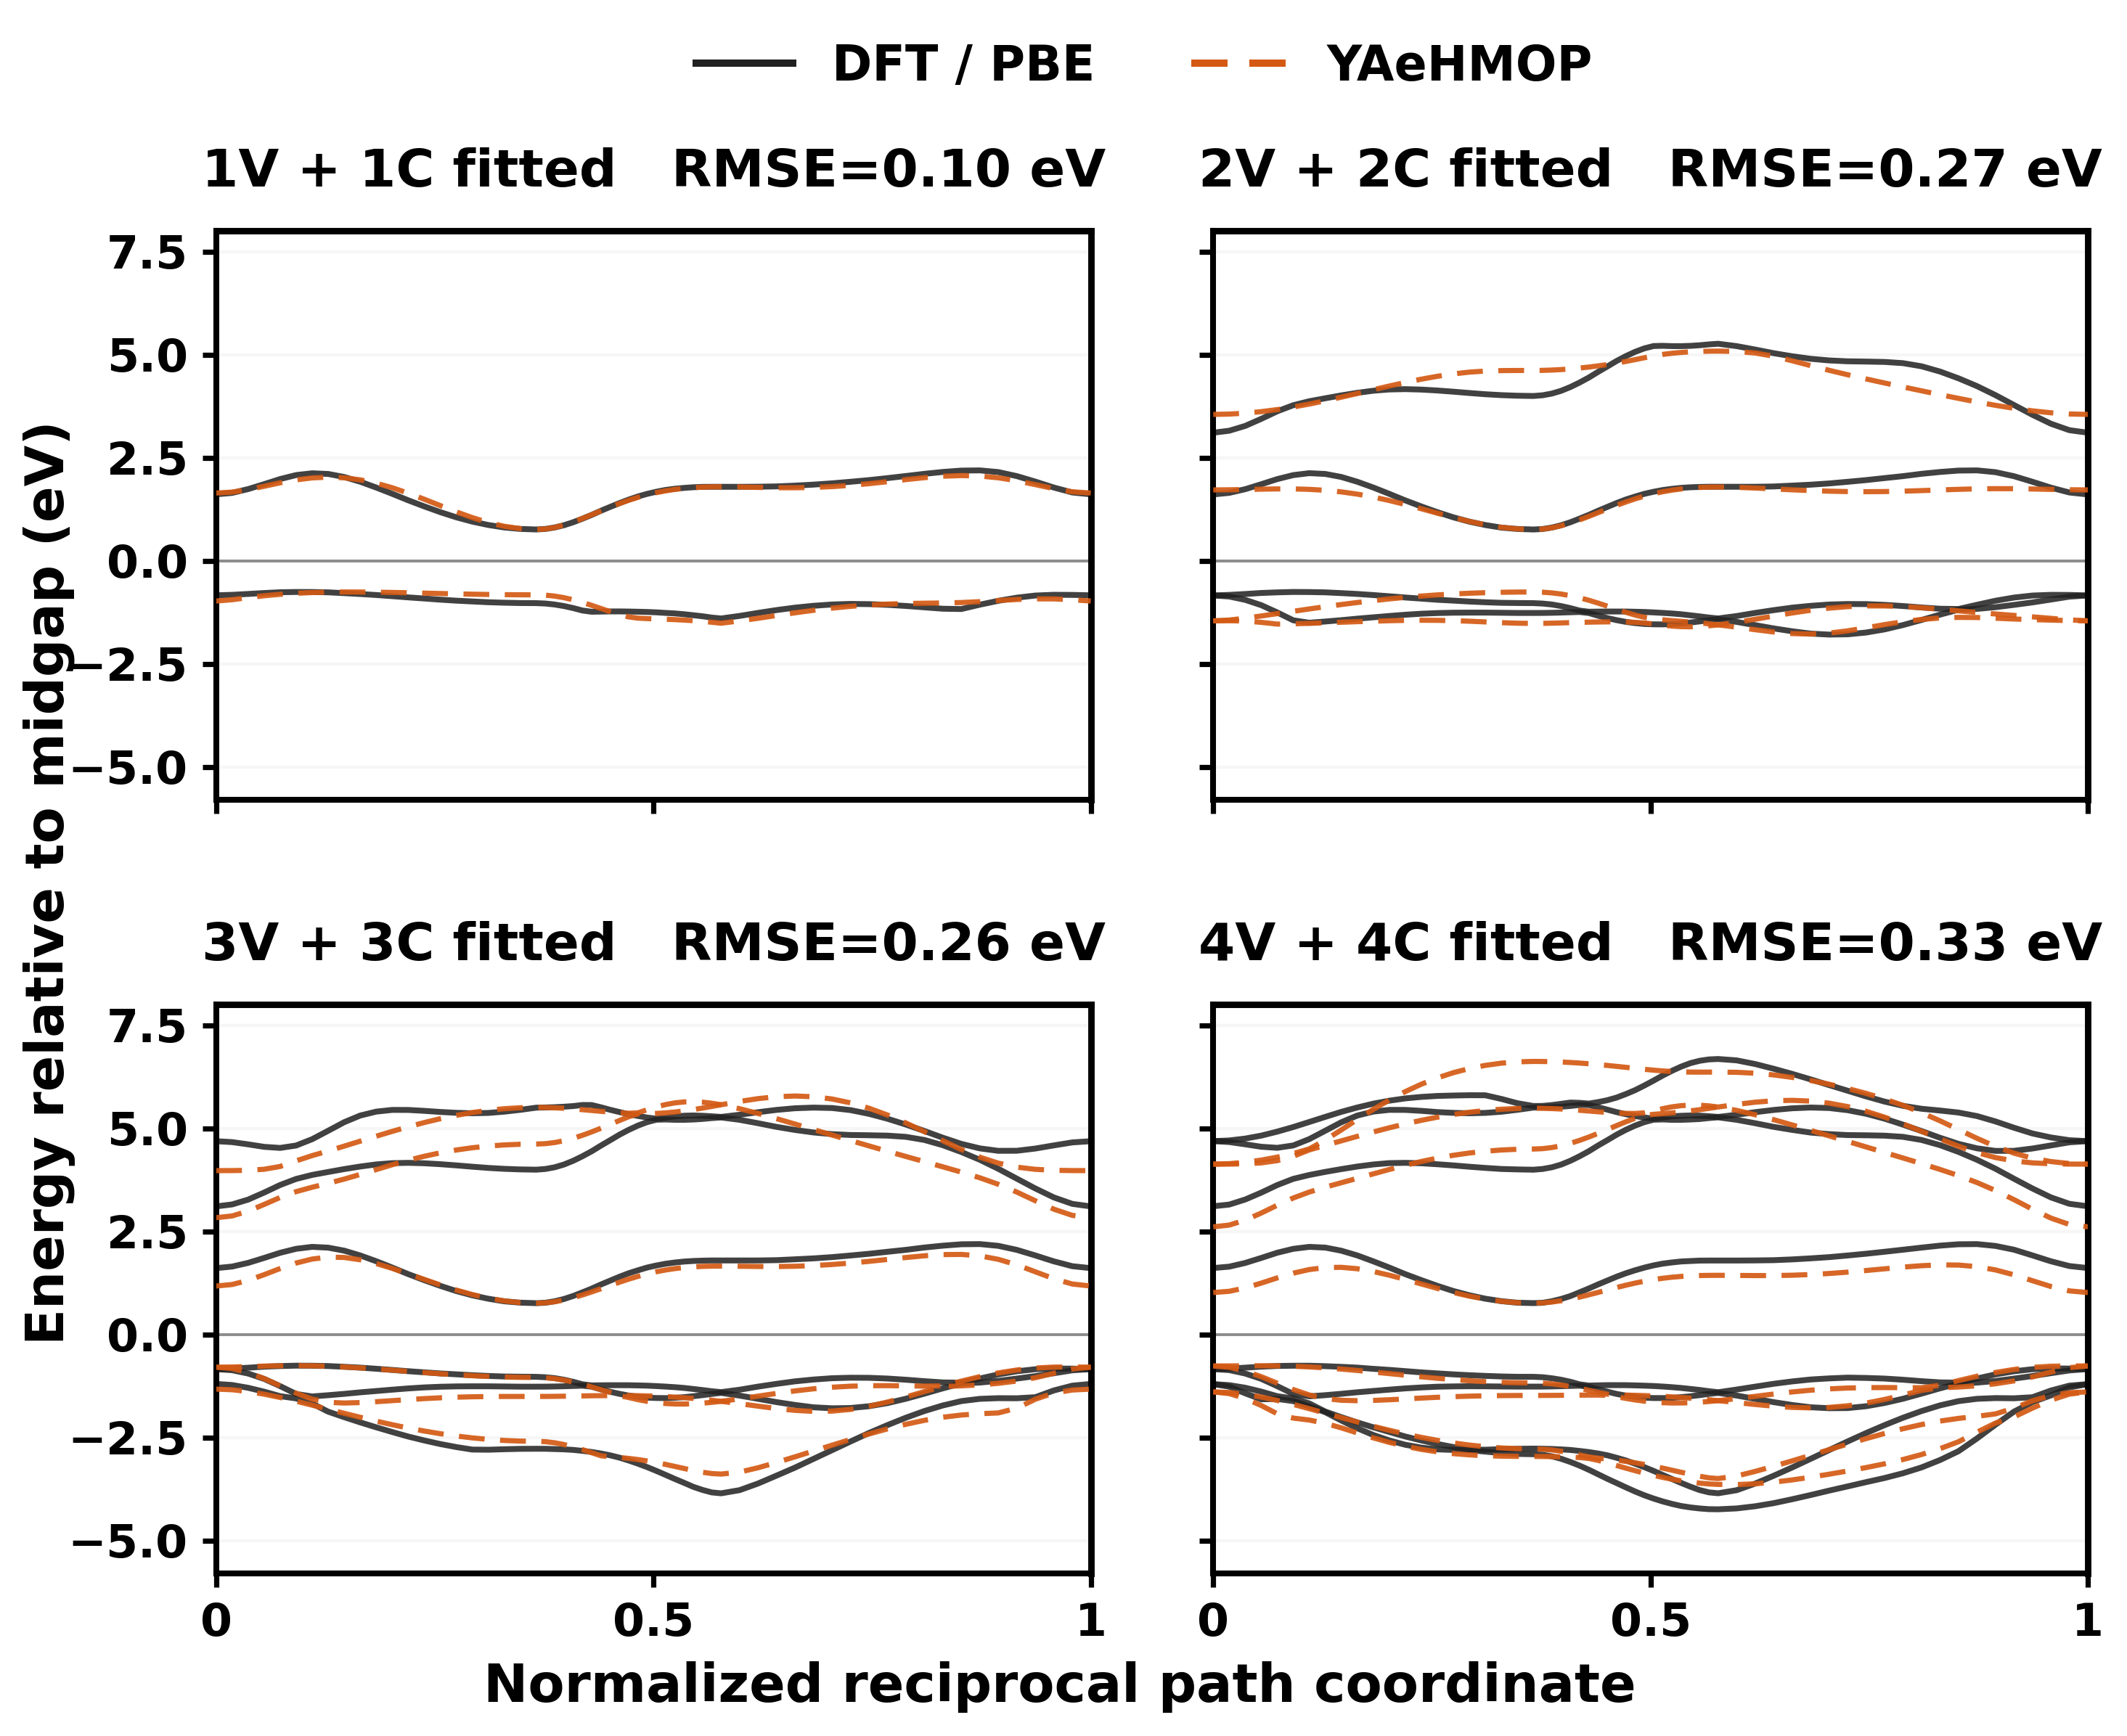
\includegraphics[width=0.78\textwidth]{paper_fig04_SnS2.png}
\caption{SnS$_2$, paper figure 4: PBE (black) and fitted YAeHMOP bands (orange) for 2, 4, 6 and 8
matched bands. RMSE 0.1043, 0.2725, 0.2561 and 0.3333 eV.}
\end{figure}

\begin{center}
\begin{tabular}{lrrrr}
\toprule
Direct-fit RMSE (eV) & 2 (1V+1C) & 4 (2V+2C) & 6 (3V+3C) & 8 (4V+4C) \\
\midrule
GeS   & 0.3323 & 0.3395 & 0.3282 & 0.4515 \\
GeSe  & 0.2514 & 0.2138 & 0.2243 & 0.2526 \\
GeTe  & 0.2716 & 0.2977 & 0.2929 & n/a \\
SnS$_2$ & \textbf{0.1043} & 0.2725 & 0.2561 & 0.3333 \\
SnSe  & 0.2679 & 0.2265 & 0.3189 & 0.3222 \\
SnTe  & 0.1482 & \textbf{0.1391} & \textbf{0.2191} & \textbf{0.2433} \\
\midrule
Mean direct fit & 0.229 & 0.248 & 0.273 & 0.321 \\
Mean whole-compound held out & 0.807 & 0.909 & 0.704 & 3.416 \\
\bottomrule
\end{tabular}
\end{center}

GeTe has no eligible eight-band window. The held-out means use 6, 6, 6 and 4 folds. The carbon
extensions (graphene, phagraphene, diamond, graphite) use other PBE sources and are described in
\cmd{docs/BEST\_RESULTS.md}; numbers from different references must not be averaged together.

% ================================================================ 10
\section{Scope and limitations}

\begin{itemize}
  \item Only \textbf{gapped, nonmagnetic, spinless} references: the fitter rejects frontier gaps below
        about 0.02 eV and odd electron counts. Graphene's Dirac crossing, metals, spin-polarized and
        spin--orbit split bands need other objectives.
  \item A band path is a one-dimensional cut: it does not establish Fermi-surface topology, DOS or
        forces.
  \item A direct fit is a calibration. Transfer claims need frozen or family evaluation on materials
        excluded from fitting.
  \item Images cannot reveal hidden or overlapping bands; prefer the original numerical bands.
  \item The reference must match the CIF, the k path and the energy axis. Record the DFT functional,
        basis or pseudopotential, k mesh, spin/SOC treatment, YAeHMOP version, $K$, exponents, on-site
        energies and number of images.
  \item The optimizer gives no guarantee of a global minimum; repeat with other seeds or larger budgets
        to check convergence.
\end{itemize}

% ================================================================ 11
\section{Command reference: \cmd{bands\_fit.py}}

\begin{center}
\small
\begin{tabularx}{\textwidth}{>{\ttfamily}l L}
\toprule
\normalfont Flag & Meaning \\
\midrule
cif, input\_file & structure (any format of section~\ref{sec:structure}) and INI settings (positional) \\
--structure-format & force the structure format (default \cmd{auto}) \\
--dft-dir, --dft-code & raw DFT band data as reference (section~\ref{sec:dft}) \\
--dft-file, --valence-bands & band file to use; occupied DFT bands \\
--dimension & periodic dimension of a DFT reference \\
--fitting-dir & folder of the standard fit outputs (default \cmd{OUTDIR/fitting}) \\
--image, --png & reference image or CSV instead of \cmd{[reference] image} \\
--pairs \{1,2,3,4\} & valence and conduction bands on \emph{each} side \\
--mode & \cmd{auto}, \cmd{layered}, \cmd{colors}, \cmd{mono}, \cmd{csv} \\
--bbox L,T,R,B & plot interior in pixels \\
--colors & one hex color per band, in energy order \\
--allow-ambiguous & relax tracing checks (unsafe; avoid for publications) \\
--validate-only & check files and format only; no extraction, no solver \\
--prepare-only & extract, encode, preview and QA; no solver \\
--budget N & number of YAeHMOP calls ($\ge 80$; $\ge 160$ for SA/HJ refinements) \\
--optimizer NAME & fitting algorithm (section 6) \\
--polish & \cmd{nelder-mead} or \cmd{powell} after a global optimizer \\
--seed & random seed (default 20261014) \\
--from-fit fit.json & recompute all bands from a saved fit (runs the solver) \\
--from-parameters, --k & recompute all bands from your table and $K$ \\
--overlap-radius & periodic images per active direction, 1--8 (default 5) \\
--name, --outdir & label and output folder \\
\bottomrule
\end{tabularx}
\end{center}

Other tools: \cmd{prepare\_band\_png.py} (image or CSV to bitplanes; flags \cmd{--n-pairs},
\cmd{--emin}, \cmd{--emax}, \cmd{--mode}, \cmd{--bbox}, \cmd{--colors}, \cmd{--color-tolerance},
\cmd{--trace-nx}, \cmd{--min-coverage}), \cmd{inspect\_png.py}, \cmd{digitize\_bands.py},
\cmd{strategy\_advisor.py} (rule-based advice, no calculation), \cmd{scripts/plot\_saved\_bands.py} and
\cmd{scripts/recompute\_carbon.py}. Each has \cmd{--help}.

% ================================================================ 12
\section{Troubleshooting}

\begin{center}
\small
\begin{tabularx}{\textwidth}{>{\raggedright\arraybackslash}p{4.6cm} L}
\toprule
Symptom & Cause and remedy \\
\midrule
\cmd{No module named ase/numpy/...} & activate the environment and install the requirements \\
\cmd{YAeHMOP bind not found} & set \cmd{YAEHMOP\_BIND} and \cmd{YAEHMOP\_PARAM\_FILE}; \cmd{--prepare-only} does not need them \\
CSV \cmd{header must be exactly} & use \cmd{x,band\_1,band\_2,...}, energies ascending per row \\
\cmd{CSV energy extends beyond emin/emax} & widen \cmd{emin}/\cmd{emax} or shift the reference \\
\cmd{N reliable curve colors were not found} & give \cmd{--colors}, or use a CSV or manual annotations \\
\cmd{Invalid band gap} & gapless or metallic reference: not supported by this objective \\
\cmd{Invalid or out-of-range plot box} & \cmd{--bbox} must lie inside the oriented, normalized image \\
\cmd{needs scikit-learn} / \cmd{needs the cma package} & install the optional package or use the conda environment \\
3D crystal treated as 2D & set \cmd{dimension = 3}; refit fits made before the periodicity fix \\
\bottomrule
\end{tabularx}
\end{center}

\section*{Credits}
YAeHMOP: G.~A.~Landrum and W.~V.~Glassey (\url{https://github.com/greglandrum/yaehmop}). ASE, SciPy,
scikit-learn and \cmd{cma} are used under their own licenses. This front-end is MIT licensed; external
PBE data keep their own licenses and are not redistributed.

\end{document}
